\chapter{Network Framework}\label{ch:Network Framework}
Completing the second part of the project requires implementing the Speech Recogniser in a distributed manner. High level, the system requires open access over a network, local or otherwise. Low level, the recognizer must be able to communicate over the available network. In order to demonstrate the system's complete functionality, a Virtual Private Network (VPN) is used to provide open access between devices and sockets are used to send data through the network.

\section{Virtual Private Network (VPN)}
The VPN extends a private network over a public network and enables devices to send and receive data across shared or public networks, in the same way as if they would be directly connected to the same network. 
Due to the fact that multiple devices are in various locations and on different networks, some of which have security protocols enabled, direct communication between these devices is not possible without a VPN.\\\\
OpenVPN is the open-source software application that was utilized here. 
It implements VPN techniques for creating secure point-to-point connections in routed or bridged configurations and remote access. 
A custom security protocol, based on SSL/TLS is enforced on the network, and it is capable of traversing network address translators (NATs) and firewalls.\\\\
For the current project, OpenVPN was used in a multiclient-server configuration. The server itself was installed on a Raspberry Pi 3.
Authentication certificates were released for every client that required access to the network \cite{OpnVPN}.
The network setup is shown in Figure \ref{fig:vpn_uni_diagram}.
\begin{figure}[H]
    \centering
    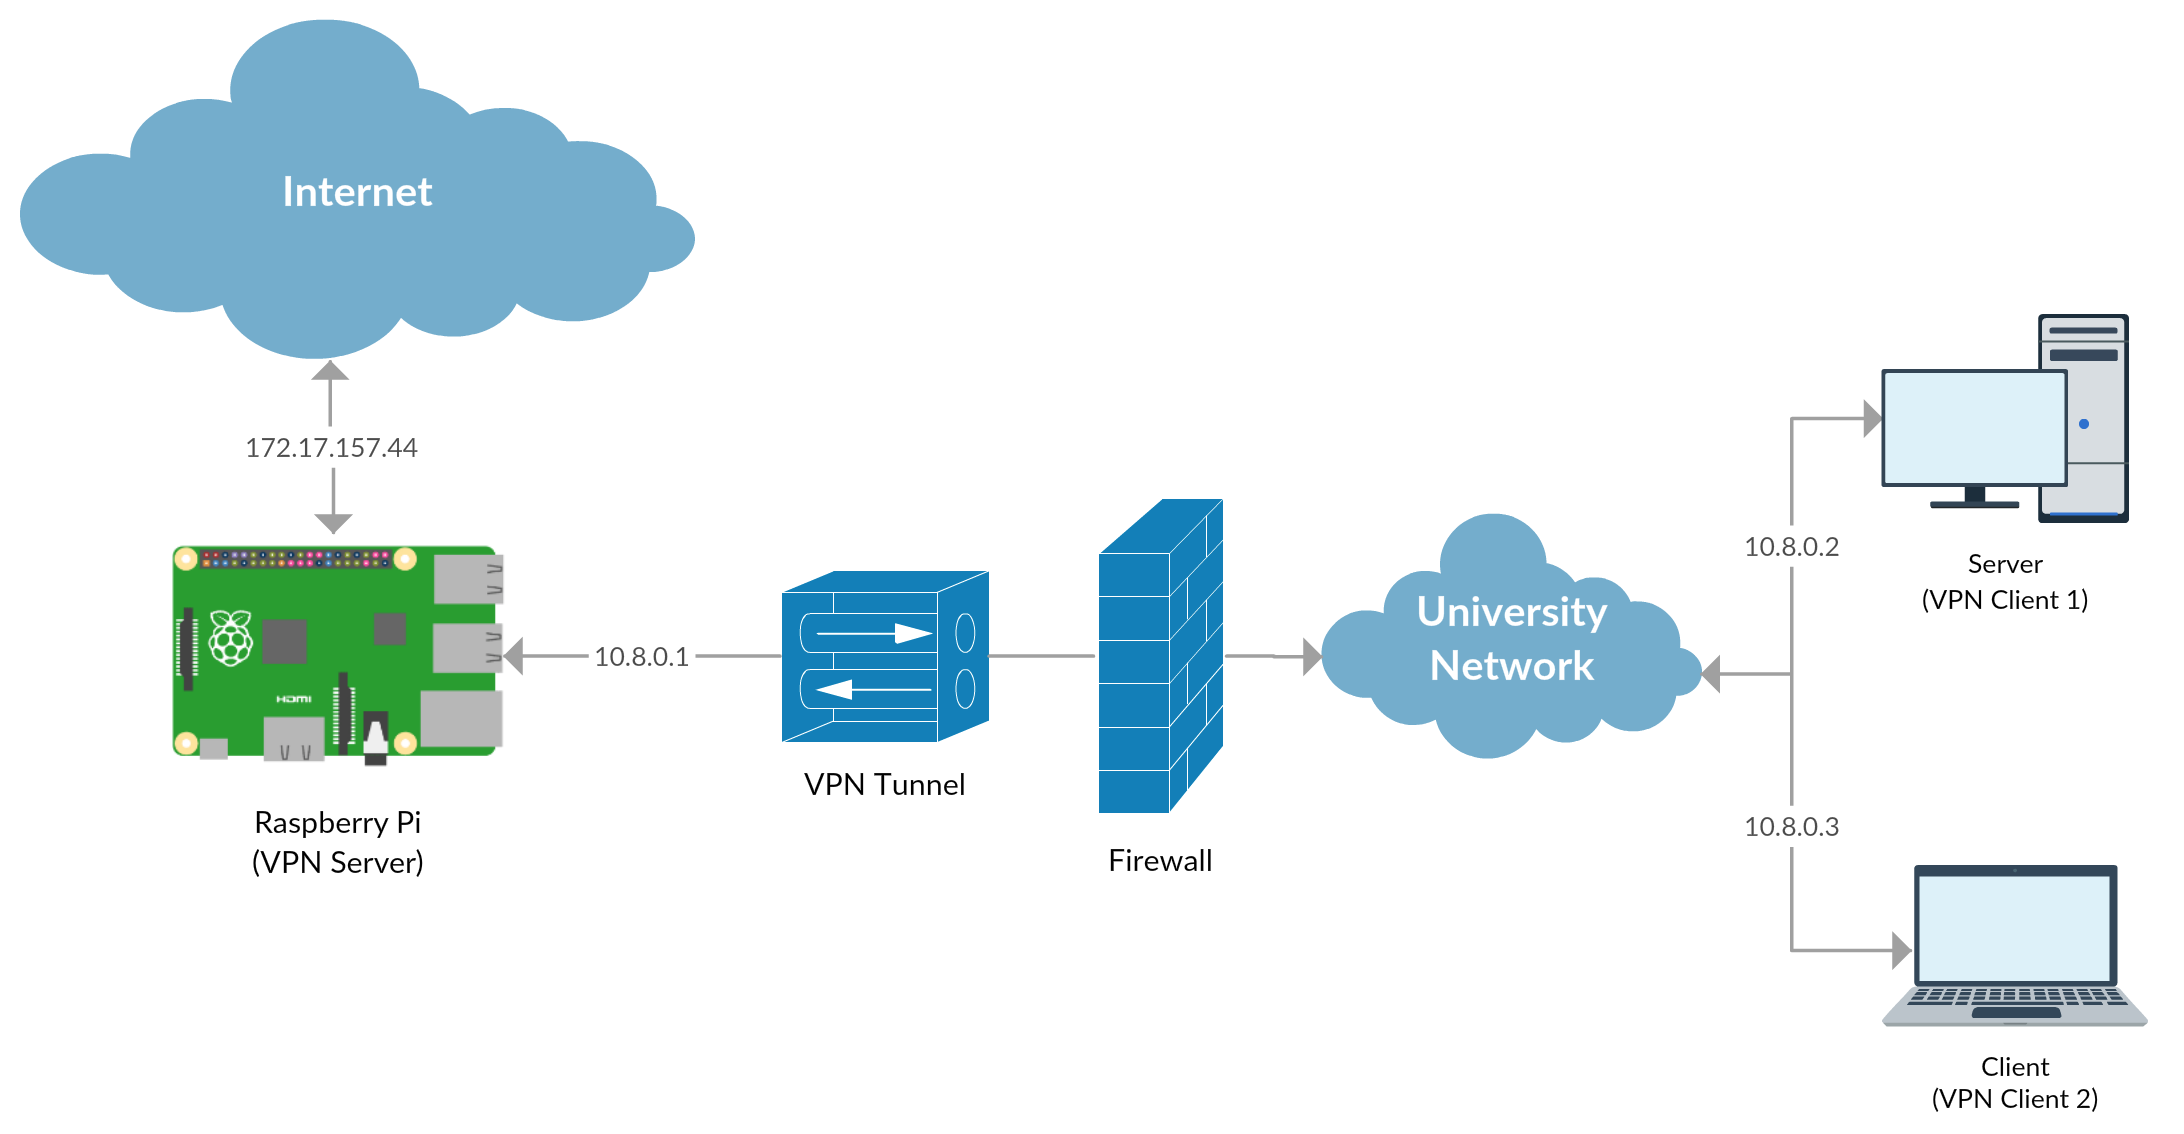
\includegraphics[width=.9\textwidth]        
    {network_framework/client_server_framework}
    \caption{Virtual private network to university.}
    \label{fig:vpn_uni_diagram}
\end{figure}

\section{Sockets}
Network sockets are software interfaces that allow communication between two different processes on the same or on different machines.
Most often utilized in client-server frameworks, a network socket represents one endpoint in a communication flow between two programs.\\\\
In this project, TCP sockets were implemented in Python to provide support for a variety of desktop-based operating systems.
When the server is initialized, it creates a socket and listens for incoming requests.
\begin{lstlisting}[language=Python, flexiblecolumns=true, caption=Server initialization.]
(HOST,PORT) = (server_ip,port)
s = socket.socket(socket.AF_INET, socket.SOCK_STREAM)
s.bind((HOST, PORT))
s.listen(numb_of_clients)
return s
\end{lstlisting}
On the client side, another TCP socket is created and using the server's IP address and port number, a connection is established. 
\begin{lstlisting}[language=Python, flexiblecolumns=true, caption=Client initialization.]
(HOST,PORT)=('10.8.0.2',2001)
s=socket.socket(socket.AF_INET,socket.SOCK_STREAM);
s.connect((HOST,PORT))
\end{lstlisting}
Following a successful connection, the client sends audio information to the server, which will return the decoded data in text form. 